\documentclass{ximera}

%\usepackage{todonotes}

\newcommand{\todo}{}

\usepackage{esint} % for \oiint
\ifxake%%https://math.meta.stackexchange.com/questions/9973/how-do-you-render-a-closed-surface-double-integral
\renewcommand{\oiint}{{\large\bigcirc}\kern-1.56em\iint}
\fi


\graphicspath{
  {./}
  {ximeraTutorial/}
  {basicPhilosophy/}
  {functionsOfSeveralVariables/}
  {normalVectors/}
  {lagrangeMultipliers/}
  {vectorFields/}
  {greensTheorem/}
  {shapeOfThingsToCome/}
  {dotProducts/}
  {partialDerivativesAndTheGradientVector/}
  {../productAndQuotientRules/exercises/}
  {../normalVectors/exercisesParametricPlots/}
  {../continuityOfFunctionsOfSeveralVariables/exercises/}
  {../partialDerivativesAndTheGradientVector/exercises/}
  {../directionalDerivativeAndChainRule/exercises/}
  {../commonCoordinates/exercisesCylindricalCoordinates/}
  {../commonCoordinates/exercisesSphericalCoordinates/}
  {../greensTheorem/exercisesCurlAndLineIntegrals/}
  {../greensTheorem/exercisesDivergenceAndLineIntegrals/}
  {../shapeOfThingsToCome/exercisesDivergenceTheorem/}
  {../greensTheorem/}
  {../shapeOfThingsToCome/}
  {../separableDifferentialEquations/exercises/}
  {vectorFields/}
}

\newcommand{\mooculus}{\textsf{\textbf{MOOC}\textnormal{\textsf{ULUS}}}}

\usepackage{tkz-euclide}
\usepackage{tikz}
\usepackage{tikz-cd}
\usetikzlibrary{arrows}
\tikzset{>=stealth,commutative diagrams/.cd,
  arrow style=tikz,diagrams={>=stealth}} %% cool arrow head
\tikzset{shorten <>/.style={ shorten >=#1, shorten <=#1 } } %% allows shorter vectors

\usetikzlibrary{backgrounds} %% for boxes around graphs
\usetikzlibrary{shapes,positioning}  %% Clouds and stars
\usetikzlibrary{matrix} %% for matrix
\usepgfplotslibrary{polar} %% for polar plots
\usepgfplotslibrary{fillbetween} %% to shade area between curves in TikZ
%\usetkzobj{all}
\usepackage[makeroom]{cancel} %% for strike outs
%\usepackage{mathtools} %% for pretty underbrace % Breaks Ximera
%\usepackage{multicol}
\usepackage{pgffor} %% required for integral for loops



%% http://tex.stackexchange.com/questions/66490/drawing-a-tikz-arc-specifying-the-center
%% Draws beach ball
\tikzset{pics/carc/.style args={#1:#2:#3}{code={\draw[pic actions] (#1:#3) arc(#1:#2:#3);}}}



\usepackage{array}
\setlength{\extrarowheight}{+.1cm}
\newdimen\digitwidth
\settowidth\digitwidth{9}
\def\divrule#1#2{
\noalign{\moveright#1\digitwidth
\vbox{\hrule width#2\digitwidth}}}




% \newcommand{\RR}{\mathbb R}
% \newcommand{\R}{\mathbb R}
% \newcommand{\N}{\mathbb N}
% \newcommand{\Z}{\mathbb Z}

\newcommand{\sagemath}{\textsf{SageMath}}


%\renewcommand{\d}{\,d\!}
%\renewcommand{\d}{\mathop{}\!d}
%\newcommand{\dd}[2][]{\frac{\d #1}{\d #2}}
%\newcommand{\pp}[2][]{\frac{\partial #1}{\partial #2}}
% \renewcommand{\l}{\ell}
%\newcommand{\ddx}{\frac{d}{\d x}}

% \newcommand{\zeroOverZero}{\ensuremath{\boldsymbol{\tfrac{0}{0}}}}
%\newcommand{\inftyOverInfty}{\ensuremath{\boldsymbol{\tfrac{\infty}{\infty}}}}
%\newcommand{\zeroOverInfty}{\ensuremath{\boldsymbol{\tfrac{0}{\infty}}}}
%\newcommand{\zeroTimesInfty}{\ensuremath{\small\boldsymbol{0\cdot \infty}}}
%\newcommand{\inftyMinusInfty}{\ensuremath{\small\boldsymbol{\infty - \infty}}}
%\newcommand{\oneToInfty}{\ensuremath{\boldsymbol{1^\infty}}}
%\newcommand{\zeroToZero}{\ensuremath{\boldsymbol{0^0}}}
%\newcommand{\inftyToZero}{\ensuremath{\boldsymbol{\infty^0}}}



% \newcommand{\numOverZero}{\ensuremath{\boldsymbol{\tfrac{\#}{0}}}}
% \newcommand{\dfn}{\textbf}
% \newcommand{\unit}{\,\mathrm}
% \newcommand{\unit}{\mathop{}\!\mathrm}
% \newcommand{\eval}[1]{\bigg[ #1 \bigg]}
% \newcommand{\seq}[1]{\left( #1 \right)}
% \renewcommand{\epsilon}{\varepsilon}
% \renewcommand{\phi}{\varphi}


% \renewcommand{\iff}{\Leftrightarrow}

% \DeclareMathOperator{\arccot}{arccot}
% \DeclareMathOperator{\arcsec}{arcsec}
% \DeclareMathOperator{\arccsc}{arccsc}
% \DeclareMathOperator{\si}{Si}
% \DeclareMathOperator{\scal}{scal}
% \DeclareMathOperator{\sign}{sign}


%% \newcommand{\tightoverset}[2]{% for arrow vec
%%   \mathop{#2}\limits^{\vbox to -.5ex{\kern-0.75ex\hbox{$#1$}\vss}}}
% \newcommand{\arrowvec}[1]{{\overset{\rightharpoonup}{#1}}}
% \renewcommand{\vec}[1]{\arrowvec{\mathbf{#1}}}
% \renewcommand{\vec}[1]{{\overset{\boldsymbol{\rightharpoonup}}{\mathbf{#1}}}}

% \newcommand{\point}[1]{\left(#1\right)} %this allows \vector{ to be changed to \vector{ with a quick find and replace
% \newcommand{\pt}[1]{\mathbf{#1}} %this allows \vec{ to be changed to \vec{ with a quick find and replace
% \newcommand{\Lim}[2]{\lim_{\point{#1} \to \point{#2}}} %Bart, I changed this to point since I want to use it.  It runs through both of the exercise and exerciseE files in limits section, which is why it was in each document to start with.

% \DeclareMathOperator{\proj}{\mathbf{proj}}
% \newcommand{\veci}{{\boldsymbol{\hat{\imath}}}}
% \newcommand{\vecj}{{\boldsymbol{\hat{\jmath}}}}
% \newcommand{\veck}{{\boldsymbol{\hat{k}}}}
% \newcommand{\vecl}{\vec{\boldsymbol{\l}}}
% \newcommand{\uvec}[1]{\mathbf{\hat{#1}}}
% \newcommand{\utan}{\mathbf{\hat{t}}}
% \newcommand{\unormal}{\mathbf{\hat{n}}}
% \newcommand{\ubinormal}{\mathbf{\hat{b}}}

% \newcommand{\dotp}{\bullet}
% \newcommand{\cross}{\boldsymbol\times}
% \newcommand{\grad}{\boldsymbol\nabla}
% \newcommand{\divergence}{\grad\dotp}
% \newcommand{\curl}{\grad\cross}
%\DeclareMathOperator{\divergence}{divergence}
%\DeclareMathOperator{\curl}[1]{\grad\cross #1}
% \newcommand{\lto}{\mathop{\longrightarrow\,}\limits}

% \renewcommand{\bar}{\overline}

\colorlet{textColor}{black}
\colorlet{background}{white}
\colorlet{penColor}{blue!50!black} % Color of a curve in a plot
\colorlet{penColor2}{red!50!black}% Color of a curve in a plot
\colorlet{penColor3}{red!50!blue} % Color of a curve in a plot
\colorlet{penColor4}{green!50!black} % Color of a curve in a plot
\colorlet{penColor5}{orange!80!black} % Color of a curve in a plot
\colorlet{penColor6}{yellow!70!black} % Color of a curve in a plot
\colorlet{fill1}{penColor!20} % Color of fill in a plot
\colorlet{fill2}{penColor2!20} % Color of fill in a plot
\colorlet{fillp}{fill1} % Color of positive area
\colorlet{filln}{penColor2!20} % Color of negative area
\colorlet{fill3}{penColor3!20} % Fill
\colorlet{fill4}{penColor4!20} % Fill
\colorlet{fill5}{penColor5!20} % Fill
\colorlet{gridColor}{gray!50} % Color of grid in a plot

\newcommand{\surfaceColor}{violet}
\newcommand{\surfaceColorTwo}{redyellow}
\newcommand{\sliceColor}{greenyellow}




\pgfmathdeclarefunction{gauss}{2}{% gives gaussian
  \pgfmathparse{1/(#2*sqrt(2*pi))*exp(-((x-#1)^2)/(2*#2^2))}%
}


%%%%%%%%%%%%%
%% Vectors
%%%%%%%%%%%%%

%% Simple horiz vectors
\renewcommand{\vector}[1]{\left\langle #1\right\rangle}


%% %% Complex Horiz Vectors with angle brackets
%% \makeatletter
%% \renewcommand{\vector}[2][ , ]{\left\langle%
%%   \def\nextitem{\def\nextitem{#1}}%
%%   \@for \el:=#2\do{\nextitem\el}\right\rangle%
%% }
%% \makeatother

%% %% Vertical Vectors
%% \def\vector#1{\begin{bmatrix}\vecListA#1,,\end{bmatrix}}
%% \def\vecListA#1,{\if,#1,\else #1\cr \expandafter \vecListA \fi}

%%%%%%%%%%%%%
%% End of vectors
%%%%%%%%%%%%%

%\newcommand{\fullwidth}{}
%\newcommand{\normalwidth}{}



%% makes a snazzy t-chart for evaluating functions
%\newenvironment{tchart}{\rowcolors{2}{}{background!90!textColor}\array}{\endarray}

%%This is to help with formatting on future title pages.
\newenvironment{sectionOutcomes}{}{}



%% Flowchart stuff
%\tikzstyle{startstop} = [rectangle, rounded corners, minimum width=3cm, minimum height=1cm,text centered, draw=black]
%\tikzstyle{question} = [rectangle, minimum width=3cm, minimum height=1cm, text centered, draw=black]
%\tikzstyle{decision} = [trapezium, trapezium left angle=70, trapezium right angle=110, minimum width=3cm, minimum height=1cm, text centered, draw=black]
%\tikzstyle{question} = [rectangle, rounded corners, minimum width=3cm, minimum height=1cm,text centered, draw=black]
%\tikzstyle{process} = [rectangle, minimum width=3cm, minimum height=1cm, text centered, draw=black]
%\tikzstyle{decision} = [trapezium, trapezium left angle=70, trapezium right angle=110, minimum width=3cm, minimum height=1cm, text centered, draw=black]


\title{Trigonometric}

\begin{document}

\begin{abstract}
sine and cosine
\end{abstract}
\maketitle















\section*{The Unit Circle}


The \textbf{unit circle} is the circle of radius $1$ centered at the origin on the Cartesian plane. The points on the unit cricle have two coordinates.  

\begin{itemize}
\item The first coordinate gives the horizontal position of the point. 
\item The second coordinate gives the vertical position of the point.  
\end{itemize}

Both of these depend on an angle measurement, $\theta$. This angle, $\theta$, is the angle made between the horizontal axis and the radius running from the point on the unit circle to the origin (center of the circle).


\textbf{\textcolor{red!90!darkgray}{$\blacktriangleright$}}  The coordinates are functions of the angle!

We call these functions \textbf{cosine} and \textbf{sine}.



\begin{image}
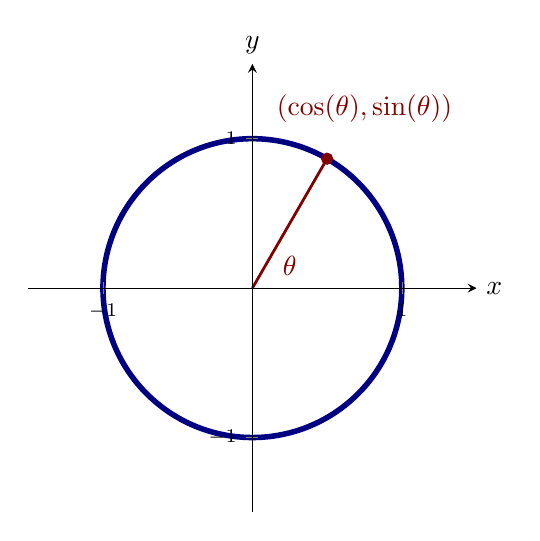
\begin{tikzpicture} 
  \begin{axis}[
            domain=-1.5:1.5, ymax=1.5, xmax=1.5, ymin=-1.5, xmin=-1.5,
            axis lines =center, unit vector ratio*=1 1 1, xlabel=$x$, ylabel=$y$,
            ticklabel style={font=\scriptsize},
            every axis y label/.style={at=(current axis.above origin),anchor=south},
            every axis x label/.style={at=(current axis.right of origin),anchor=west},
            axis on top
          ]
          
          	\addplot [line width=2, penColor, smooth,samples=100,domain=(0:6.3)] ({cos(deg(x))},{sin(deg(x)});


        	\addplot [color=penColor2,only marks,mark=*] coordinates{(0.5,0.866)};


        	%\draw[decoration={brace,raise=.2cm,mirror},decorate,thin] (axis cs:0.75,0)--(axis cs:0.75,0.866);
        	%\draw[decoration={brace,raise=.2cm},decorate,thin] (axis cs:0,0.95)--(axis cs:0.75,0.95);
        	%\node[anchor=east] at (axis cs:1.85,3) {$d$};
        	%\node[anchor=east] at (axis cs:4.6,1) {$f(d)$};
                     
        	\node at (axis cs:0.75,1.2) [penColor2] {$(\cos(\theta),\sin(\theta))$};


          \addplot [line width=1, penColor2, smooth,samples=100,domain=(0:0.5)] ({x},{1.7320*x});
          \node at (axis cs:0.25,0.15) [penColor2] {$\theta$};


          %\addplot [color=penColor,only marks,mark=*] coordinates{(-4,-1) (0,1) (1,-6.5) (7,-3.5)};

          %\addplot [line width=1, penColor2, smooth,samples=100,domain=(-4:0)] ({x},{0});
          %\addplot [line width=1, penColor2, smooth,samples=100,domain=(1:7)] ({x},{0});
           

  \end{axis}
\end{tikzpicture}
\end{image}







\subsection{Cosine}

The value of the cosine function is the horizontal coordinate of the point on the unit circle at the given angle, $\theta$. Cosine is a function of the angle $\theta$.  The shorthand for this function looks like $\cos(\theta)$. 


When we graph the cosine function the horizontal axis is measuring the angle $\theta$, since that is the domain of cosine.

\textbf{Note:}  all of our angle measurements are in radians.





\begin{image}
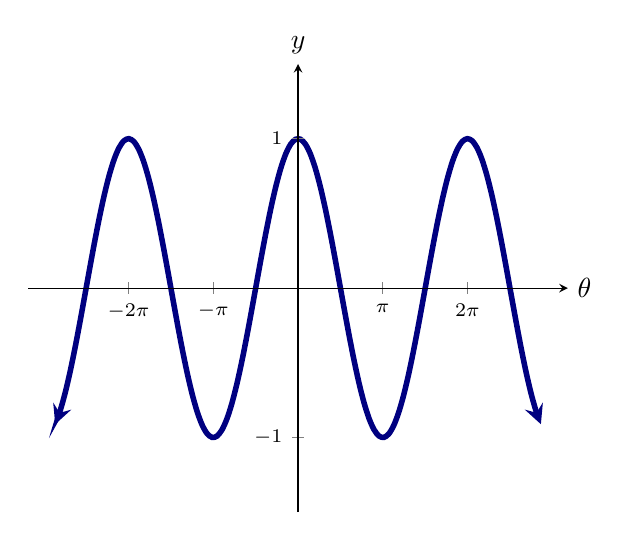
\begin{tikzpicture} 
  \begin{axis}[
            domain=-10:10, ymax=1.5, xmax=10, ymin=-1.5, xmin=-10,
            xtick={-6.28, -3.14, 3.14, 6.28}, 
            xticklabels={$-2\pi$, $-\pi$, $\pi$, $2\pi$},
            axis lines =center,  xlabel={$\theta$}, ylabel=$y$,
            ticklabel style={font=\scriptsize},
            every axis y label/.style={at=(current axis.above origin),anchor=south},
            every axis x label/.style={at=(current axis.right of origin),anchor=west},
            axis on top
          ]
          
          	\addplot [line width=2, penColor, smooth,samples=100,domain=(-9:9), <->] {cos(deg(x))};

           

  \end{axis}
\end{tikzpicture}
\end{image}



As $\theta$ rotates counterclockwise around the unit circle, the corresponding point on the unit circle moves counterclockwise and its horizontal coordinate oscillates between $-1$ and $1$.

\begin{itemize}
\item At $\theta = 0$, the horizontal coordinate is $1$. The point is on the far right of the unit circle.
\item At $\theta = \frac{\pi}{2}$, the horizontal coordinate is $0$. The point is on the top of the unit circle.
\item At $\theta = \pi$, the horizontal coordinate is $-1$. The point is on the far left of the unit circle.
\item At $\theta = \frac{3\pi}{2}$, the horizontal coordinate is $0$. The point is on the bottom of the unit circle.
\item At $\theta = 2\pi$, the horizontal coordinate is $1$. The point is again on the far right of the unit circle.
\end{itemize}


This pattern continues as $\theta \rightarrow \infty$ or the reverse, as $\theta \rightarrow -\infty$

The zeros of $\cos(\theta)$ occur at angles that place the corresponding point at the top or the bottom of the unit circle.  


\[     \cdots -\frac{5\pi}{2},  -\frac{3\pi}{2},  -\frac{\pi}{2},  \frac{\pi}{2},  \frac{3\pi}{2},  \frac{5\pi}{2} \cdots \]


There are an infinite number of zeros for cosine.  We can describe this set as follows


\[  \left\{     \frac{(2k+1)\pi}{2}          \right\}    \text{ where }  k  \text{ is any integer.}     \]





$\cos(\theta)$ has a maximum value of $1$, which occurs at every even $\pi$:  
\[ \{  2 \, k \, \pi \, | \, k \in \textbf{Z}\} \]



$\cos(\theta)$ has a minimum value of $-1$, which occurs at every odd $\pi$:  
\[ \{  (2k+1) \, \pi \, | \, k \in \textbf{Z}\} \]











\subsection*{Sine}

The value of the function is the vertical coordinate of the point on the unit circle at the given angle. Sine is a function of the angle $\theta$. The shorthand for this function loks like $\sin(\theta)$. 



When we graph the sine function the horizontal axis is measuring the angle $\theta$, since that is the domain of sine.

\textbf{Note:}  all of our angle measurements are in radians.





\begin{image}
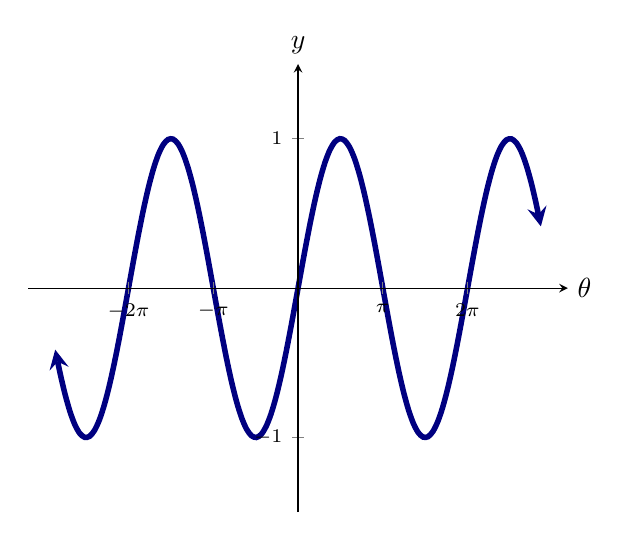
\begin{tikzpicture} 
  \begin{axis}[
            domain=-10:10, ymax=1.5, xmax=10, ymin=-1.5, xmin=-10,
            xtick={-6.28, -3.14, 3.14, 6.28}, 
            xticklabels={$-2\pi$, $-\pi$, $\pi$, $2\pi$},
            axis lines =center,  xlabel={$\theta$}, ylabel=$y$,
            ticklabel style={font=\scriptsize},
            every axis y label/.style={at=(current axis.above origin),anchor=south},
            every axis x label/.style={at=(current axis.right of origin),anchor=west},
            axis on top
          ]
          
          	\addplot [line width=2, penColor, smooth,samples=100,domain=(-9:9), <->] {sin(deg(x))};

           

  \end{axis}
\end{tikzpicture}
\end{image}



As $\theta$ rotates counterclockwise, the corresponding point on the unit circle moves counterclockwise and its vertical coordinate oscillates between $-1$ and $1$.

\begin{itemize}
\item At $\theta = 0$, the vertical coordinate is $0$. The point is on the far right of the unit circle.
\item At $\theta = \frac{\pi}{2}$, the vertical coordinate is $1$. The point is on the top of the unit circle.
\item At $\theta = \pi$, the vertical coordinate is $0$. The point is on the far left of the unit circle.
\item At $\theta = \frac{3\pi}{2}$, the vertical coordinate is $-1$. The point is on the bottom of the unit circle.
\item At $\theta = 2\pi$, the vertical coordinate is $0$. The point is again on the far right of the unit circle.
\end{itemize}


This pattern continues as $\theta \rightarrow \infty$ or the reverse, as $\theta \rightarrow -\infty$

The zeros of $\sin(\theta)$ occur at angles that place the corresponding point at the left and right of the unit circle.  


\[     \cdots -2\pi, -\pi, 0, \pi, -2\pi \cdots \]


There are an infinite number of zeros for sine.  We can describe this set as follows


\[  \{  k \, \pi   \, | \, k \in \textbf{Z}   \}      \]





$\sin(\theta)$ has a maximum value of $1$, which occurs at every half $\pi$:  
\[ \left\{  \frac{(4k+1)\pi}{2} \, | \, k \in \textbf{Z}\right\} \]



$\sin(\theta)$ has a minimum value of $-1$, which occurs at every three-halves $\pi$:  
\[ \left\{  \frac{(4k+3)\pi}{2} \, | \, k \in \textbf{Z}\right\} \]











\subsection*{Tangent}


While sine and cosine are the coordinates of points on the unit circle, we have other trigonometric functions, which are built from sine and cosine.  The tangent function is the quotient of sine and cosine.




\[ \tan(\theta) = \frac{\sin(\theta)}{\cos(\theta)} \]


Everywhere that $\sin(\theta)$ has a zero, so does $\tan(\theta)$

Everywhere that $\cos(\theta)$ has a zero, $\tan(\theta)$ has a singularity.


Therefore the domain of $\tan(\theta)$ is the union of every interval between the zeros of $\cos(\theta)$.


\[      \cdots   \cup  \left(\frac{-3\pi}{2}, \frac{-\pi}{2}\right) \cup \left(\frac{-\pi}{2}, \frac{\pi}{2}\right) \cup \left(\frac{\pi}{2} , \frac{3\pi}{2}\right) \cup \cdots              \]


Of course, there is shorthand for infinite unions







\[    \bigcup^\infty_{k=-\infty} \left(\frac{(2k-1)\pi}{2}, \frac{(2k+1)\pi}{2}\right)   \]













\begin{image}
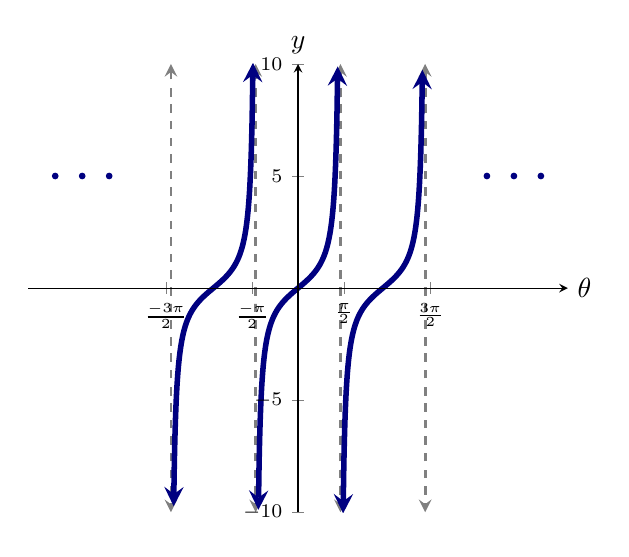
\begin{tikzpicture} 
  \begin{axis}[
            domain=-10:10, ymax=10, xmax=10, ymin=-10, xmin=-10,
            xtick={-4.9, -1.7, 1.7, 4.9}, 
            xticklabels={$\frac{-3\pi}{2}$, $\frac{-\pi}{2}$, $\frac{\pi}{2}$, $\frac{3\pi}{2}$},
            ticklabel style={font=\scriptsize},
            axis lines =center,  xlabel={$\theta$}, ylabel=$y$,
            every axis y label/.style={at=(current axis.above origin),anchor=south},
            every axis x label/.style={at=(current axis.right of origin),anchor=west},
            axis on top
          ]
 
            \addplot [line width=1, gray, dashed,samples=100,domain=(-10:10), <->] ({-4.71},{x});
            \addplot [line width=1, gray, dashed,samples=100,domain=(-10:10), <->] ({-1.57},{x});
            \addplot [line width=1, gray, dashed,samples=100,domain=(-10:10), <->] ({1.57},{x});
            \addplot [line width=1, gray, dashed,samples=100,domain=(-10:10), <->] ({4.71},{x});


          	\addplot [line width=2, penColor, smooth,samples=100,domain=(-1.47:1.47), <->] {tan(deg(x))};
          	\addplot [line width=2, penColor, smooth,samples=100,domain=(-4.61:-1.67), <->] {tan(deg(x))};
          	\addplot [line width=2, penColor, smooth,samples=100,domain=(1.67:4.61), <->] {tan(deg(x))};

			      \addplot[color=penColor,fill=penColor,only marks, mark size=1pt, mark=*] coordinates{(-9,5) (-8,5) (-7,5) (7,5) (8,5) (9,5)};




           

  \end{axis}
\end{tikzpicture}
\end{image}


















\subsection*{Calculating}

The unit circle is described by the equation $x^2 + y^2 = 1$.  From this we can calculate a few more values of sine and cosine.


When $\theta = \frac{\pi}{4}$, the the point is halfway between the axes, which puts it on the line $y=x$, which makes both coordinates equal.




\begin{image}
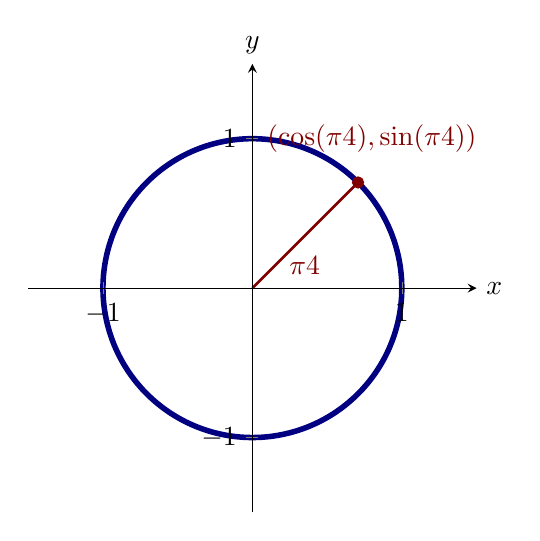
\begin{tikzpicture} 
  \begin{axis}[
            domain=-1.5:1.5, ymax=1.5, xmax=1.5, ymin=-1.5, xmin=-1.5,
            axis lines =center, unit vector ratio*=1 1 1, xlabel=$x$, ylabel=$y$,
            every axis y label/.style={at=(current axis.above origin),anchor=south},
            every axis x label/.style={at=(current axis.right of origin),anchor=west},
            axis on top
          ]
          
            \addplot [line width=2, penColor, smooth,samples=100,domain=(0:6.3)] ({cos(deg(x))},{sin(deg(x)});


          \addplot [color=penColor2,only marks,mark=*] coordinates{(0.707,0.707)};


          %\draw[decoration={brace,raise=.2cm,mirror},decorate,thin] (axis cs:0.75,0)--(axis cs:0.75,0.866);
          %\draw[decoration={brace,raise=.2cm},decorate,thin] (axis cs:0,0.95)--(axis cs:0.75,0.95);
          %\node[anchor=east] at (axis cs:1.85,3) {$d$};
          %\node[anchor=east] at (axis cs:4.6,1) {$f(d)$};
                     
          \node at (axis cs:0.8,1) [penColor2] {$(\cos(\tfrac{\pi}{4}),\sin(\tfrac{\pi}{4}))$};


          \addplot [line width=1, penColor2, smooth,samples=100,domain=(0:0.707)] {x};
          \node at (axis cs:0.35,0.15) [penColor2] {$\tfrac{\pi}{4}$};


          %\addplot [color=penColor,only marks,mark=*] coordinates{(-4,-1) (0,1) (1,-6.5) (7,-3.5)};

          %\addplot [line width=1, penColor2, smooth,samples=100,domain=(-4:0)] ({x},{0});
          %\addplot [line width=1, penColor2, smooth,samples=100,domain=(1:7)] ({x},{0});
           

  \end{axis}
\end{tikzpicture}
\end{image}




If both coordinates are equal, then our circle equation gives us 

\[   x^2 + x^2 = 1 \]

\[  2  x^2 = 1 \]

\[  x^2 = \frac{1}{2} \]


\[  \text{Either } \, x = \frac{1}{\sqrt{2}} \, \text{ or } \,  x = -\frac{1}{\sqrt{2}}   \]


Since, we are in the first quadrant, our point is $\left(\frac{1}{\sqrt{2}}, \frac{1}{\sqrt{2}}\right)$


\begin{itemize}
\item $\cos\left(\frac{\pi}{4}\right) = \frac{1}{\sqrt{2}}$ \\
\item $\sin\left(\frac{\pi}{4}\right) = \frac{1}{\sqrt{2}}$
\end{itemize}




By the symmetry of the unit circle, we can get the values for several other angles.




\begin{question}



\begin{itemize}
\item $\cos\left(\frac{3\pi}{4}\right) = \answer{-\frac{1}{\sqrt{2}}}$ \\
\item $\sin\left(\frac{3\pi}{4}\right) = \answer{\frac{1}{\sqrt{2}}}$
\end{itemize}



\end{question}





\begin{question}



\begin{itemize}
\item $\cos\left(\frac{5\pi}{4}\right) = \answer{-\frac{1}{\sqrt{2}}}$ \\
\item $\sin\left(\frac{5\pi}{4}\right) = \answer{-\frac{1}{\sqrt{2}}}$
\end{itemize}



\end{question}





\begin{question}



\begin{itemize}
\item $\cos\left(\frac{7\pi}{4}\right) = \answer{\frac{1}{\sqrt{2}}}$ \\
\item $\sin\left(\frac{7\pi}{4}\right) = \answer{-\frac{1}{\sqrt{2}}}$
\end{itemize}



\end{question}







From these, we can get the corresponding values of tangent.



\begin{question}



\begin{itemize}
\item $\tan\left(\frac{\pi}{4}\right) = \answer{1}$ \\
\item $\tan\left(\frac{3\pi}{4}\right) = \answer{-1}$ \\
\item $\tan\left(\frac{5\pi}{4}\right) = \answer{1}$ \\
\item $\tan\left(\frac{7\pi}{4}\right) = \answer{-1}$ \\
\end{itemize}



\end{question}














\begin{center}
\textbf{\textcolor{green!50!black}{ooooo-=-=-=-ooOoo-=-=-=-ooooo}} \\

more examples can be found by following this link\\ \link[More Examples of Elementary Functions]{https://ximera.osu.edu/csccmathematics/precalculus1/precalculus1/elementaryLibrary2/examples/exampleList}

\end{center}




\end{document}
